\chapter{Introduction to Control}

In chapters System modeling and Analysis, systems were modeled and analyzed by their time-response behavior by using a step function. Once the system behavior is observed and its properties defined as described in section \ref{Sec_PT2_system_properties}, sometimes most of the system properties such as its response may not be the desired response that one is looking for. In such cases system behavioral properties can be modified using a \textbf{\textit{control}}.

\section{Control Architectures}

\subsection{Open-loop control / Feedforward control} \label{Sec_OL_ControlArchitecture}

Simple to design in controls perspective given predefined disturbances and plant dynamics. The open loop control architecture can be visualized using block diagrams as shown in figure \ref{fig_OpenLoopControl}.
\begin{figure}[h!]
	\centering
	\includegraphics[width=0.8\linewidth]{Bilder/OpenLoopControl}
	\caption{Open Loop Control Architecture}
	\label{fig_OpenLoopControl}
\end{figure}
\clearpage
The control in the open loop architecture works as an inverted plant which can be explained as follows. The idea is to have output signal $Y(s)$ follow the reference signal $R(s)$. If the disturbance signal $D(s)$ is ignored the output signal of the entire system can be expressed as $Y(s) = P(s)C(s)R(s)$. If the condition that $Y(s) = R(s)$ to be met, it follows that $P(s)C(s) = 1$. If $P(s)C(s) = 1$ should be met then it follows that $C(s) := 1/P(s)$. Therefore, the control in an open-loop is just the plant inverted. This is the most simple form of control that can be applied just by inverting the plant dynamics and it requires no additional components such as sensors.

Obviously this type of design is not robust mainly because of the follows two reasons:
\begin{itemize}
	\item Model errors: It is not sometimes possible to capture the dynamics of the system perfectly or the parameters of the system would change over time or there could also be some after market changed in the system that were not previously accounted for.
	\item The disturbances to the system cannot be pre-defined accurately as this is some unknown quantity that is being influenced from the environment.
\end{itemize}
Open-loop architecture is used in the most simplified cases where the control will not be affected from external disturbances such as in washing machines where the system is isolated from the environment and the control can do its work without any external influences. Or they are also used in conjunction with feedback in complex systems as the tracking error with open-loop can be essentially eliminated to zero.

\subsection{Closed Loop Architecture / Feedback control} \label{Sec_ClosedLoopArchitecture}

Feedback control architecture will make the control system robust by using a feedback of the system outputs via a sensor. Feedback controller uses the differences between output and the reference signal to calculate the control action required to reduce the tracking error. In short feedback control works by providing a control action with respect to the error signal generated. The architecture is shown in figure \ref{fig_ClosedLoopControl}
\begin{figure}[h!]
	\centering
	\includegraphics[width=0.8\linewidth]{Bilder/ClosedLoopControl}
	\caption{Closed Loop Control Architecture}
	\label{fig_ClosedLoopControl}
\end{figure}
\newpage
One drawback of closed loop control is that it could induce instability into the system. The controller and the plant themselves my be stable on their own with negative real roots in the transfer function. But when the loop is closed the system on its whole could become unstable.

\textbf{Use of feedback: Dynamics of individual components need not be modeled}

With a feedback unlike in open-loop control, the knowledge of the individual components of the system need not be known. For example consider system shown in figure \ref{fig_Feedback_Use1}, where the position of a spindle is controlled using an electric motor.
\begin{figure}[h!]
	\centering
	\includegraphics[width=0.8\linewidth]{Bilder/Feedback_Use1}
	\caption{Use of Feedback}
	\label{fig_Feedback_Use1}
\end{figure}
It can be seen from figure \ref{fig_Feedback_Use1}, that the control on position is implemented only using the voltage to the motor as input. The individual dynamics of components such as functioning of the motor and the load inertia themselves may not even be modeled into the system. For example using a step input the response of the system can be modeled as a whole (either as PT-1 or PT-2 or the combination of both).

\textbf{Use of feedback: Make system robust and disturbance rejection}

Making a system robust is in essence successfully reject disturbance and overshadow the plant and sensor properties while controlling. For example consider a complex system as shown in figure \ref{fig_Feedback_Use2}, in order to determine what parameters the output of this system depends, a output can be determined using transfer function of the whole system:
 \begin{figure}[h!]
 	\centering
 	\includegraphics[width=0.8\linewidth]{Bilder/Feedback_Use2}
 	\caption{Use of Feedback: Making the system robust}
 	\label{fig_Feedback_Use2}
 \end{figure}

\begin{equation}
	Y(s) = F \frac{GK}{1 + GKH} r + G_d \frac{G}{1 + GKH} d_e + \frac{GKH}{1 + GKH}n
\end{equation}
when the controller gain $K$ is made significantly large, in the above equation, the following terms would take the following values:
\begin{align*}
	\frac{GK}{1 + GKH} &= 1 \\
	\frac{G}{1 + GKH} &= 0 \\
	\frac{GKH}{1 + GKH} &= 1
\end{align*}
therefore, the system output equation reduces to:
\begin{equation} \label{Eq_FeedbackUse2_Eq}
	Y(s) = F r + n
\end{equation}
From equation \eqref{Eq_FeedbackUse2_Eq}, it can be seen that when $K$ is significantly large, the response of the system becomes mostly dependent on reference TF $F$ with signal $r$ and noise signal $n$. The dynamics of plant $G$, sensor $H$ is removed from the equation, therefore the change in the dynamics of the plant or the senor will have almost no impact on the control system itself. Further the equation \eqref{Eq_FeedbackUse2_Eq} does not contain the term of disturbance $G_e$, therefore, the effect of disturbance is also rejected by the use of feedback.

\section{Block diagram reduction} \label{Sec_BlockDiagReduction}

Basically the stability or the response of the system depends on the poles. In order to be able to determine the poles of the entire system each individual blocks of the system should be reduced to form a single component system so that the transfer function and in-turn the poles of the system can be calculated easily.
\begin{figure}[h!]
	\centering
	\includegraphics[width=0.8\linewidth]{Bilder/BDR_1}
	\caption{Block diagram reduction: Algebraic}
	\label{fig_BDR_1}
\end{figure}
\begin{figure}[h!]
	\centering
	\includegraphics[width=0.8\linewidth]{Bilder/BDR_2}
	\caption{Block diagram reduction: Memorizing rules}
	\label{fig_BDR_2}
\end{figure}
\begin{figure}[h!]
	\centering
	\includegraphics[width=0.8\linewidth]{Bilder/BDR_3}
	\caption{Block diagram reduction: Series and Parallel}
	\label{fig_BDR_3}
\end{figure}
\clearpage

\section{Linearity and Principle of Superposition}

For linear systems with multiple inputs, the effect of each of the individual signals into the system can be studied separately by ignoring all other signals into the system block diagram as in linear systems the response of the system for all the inputs can later be added up to determine the overall system response as explained in a very clear detail graphically in \cite[t.41.19]{RickHill_13}.

\section{Cruise control example and drawbacks of proportional regulator}

As described in section \ref{Sec_ClosedLoopArchitecture} of closed loop architecture, once the error has been determined the controller can use this error to provide some control signal to the actuator which in-turn will reduce the tracking error. Once the error has been determined there are many ways in control theory to use this error to determine the control signal in-turn. One easiest way to calculate the control signal is by using a proportional gain regulator.

\subsection{Open-loop system model}

The cruise control system controls the traction force $F$ (or traction force is the control signal) and the tracking is required on the output velocity of the vehicle $v$. A longitudinal dynamic model of a vehicle is choose for simplicity and also noting that for a cruise control which controls only the output velocity $v$ of the vehicle, such simplified longitudinal model is sufficient. From longitudinal model it can be said that the accelerating force that is required to maintain desired $v$ can be found from Newtons second law as:
\begin{equation} \label{Eq_LongVehicleModel}
	F - F_{res} = m \dot{v}
\end{equation}
where $F$ is control signal generated to accelerate the vehicle, $F_{res}$ are the longitudinal resistance the vehicle experiences due to air drag, rolling resistance and gradient resistance, $\dot{v}$ is the vehicle acceleration and $m$ is the system parameter. Additionally, $F_{res}$ can be approximated as function of $v$ and a linear function as:
\begin{equation}
	F_{res} = b v
\end{equation}
where $b$ is a system parameter that influences $F_{res}$. Equation \ref{Eq_LongVehicleModel} becomes:
\begin{align}
	F - b v &= m \dot{v} \\
	m \dot{v} + b v = F \label{Eq_ODE_LongVehicleModel}
\end{align}
Equation \eqref{Eq_ODE_LongVehicleModel} forms the first order ODE of the longitudinal vehicle model. And the Laplace transform of equation \eqref{Eq_ODE_LongVehicleModel} is:
\begin{equation} \label{Eq_LP_ODE_VehicleModel}
	m s V(s) + b V(s) = F(s)
\end{equation}
writing in terms of transfer function:
\begin{equation} \label{Eq_TF_ODE_VehicleModel}
	\frac{V(s)}{F(s)} = \frac{1}{ms + b}
\end{equation}
writing equation \eqref{Eq_TF_ODE_VehicleModel} in canonical form:
\begin{equation}
	\frac{V(s)}{F(s)} = \frac{1/b}{\frac{m}{b}s + 1}
\end{equation}
where $k_{dc} = 1/b$ which will also give the steady-state response and $\tau = m/b$ which gives the settling time (or time constant) of the plant and $\frac{V(s)}{F(s)}$ gives the transfer function of the plant. 

\subsection{Closed Loop Model}

Now a controller with proportional gain $K$ is added in series to the plant which actuates with reference signal $R(s)$ and $V(s)$ will be the output of the entire system as shown in figure \ref{Fig_CruiseControlPRegulator}. Since this is closed loop transfer function, the block diagram reduction is shown in section \ref{Sec_BlockDiagReduction} in figure \ref{fig_BDR_2} will lead to the following system TF:
\begin{equation}
	\frac{V(s)}{R(s)} = \frac{\frac{K}{ms+b}}{1 + \frac{K}{ms+b}}
\end{equation}
simplifying the above equation leads to:
\begin{equation}
	\frac{V(s)}{R(s)} = \frac{\frac{K}{b + K}}{\frac{m}{b + K}s + 1}
\end{equation}
\begin{figure}[h!]
	\centering
	\includegraphics[width=\textwidth]{Bilder/Cruise_Control_P_Regulator.pdf}
	\caption{Block diagram of Cruise controller with P-type regulator}
	\label{Fig_CruiseControlPRegulator}
\end{figure}
therefore, $k_{dc}$ and time constant of the system are $\frac{K}{b + K}$ and $\frac{m}{b + K}$ respectively. If $K$ is chosen sufficiently larger then it will dominate the terms $k_{dc}$ and $\tau$ such that $k_{dc} \rightarrow 1$ and $\tau \rightarrow 0$ which is the most ideal case for the controller leading to perfect tracking with fast response. Additionally, the pole is at $s = \frac{-(b + K)}{m}$ and as $K$ increases the roots become more negative and this will lead to much faster response times of the controller. With no external disturbances and noise in the system the control does the tracking perfectly as shown in figure \ref{Fig_P_Regulator_Tracking}. However, a feedback loop also induces proportional noises into the system proportional to $K$ which has to be studied separately.
\begin{figure}[h!]
	\centering
	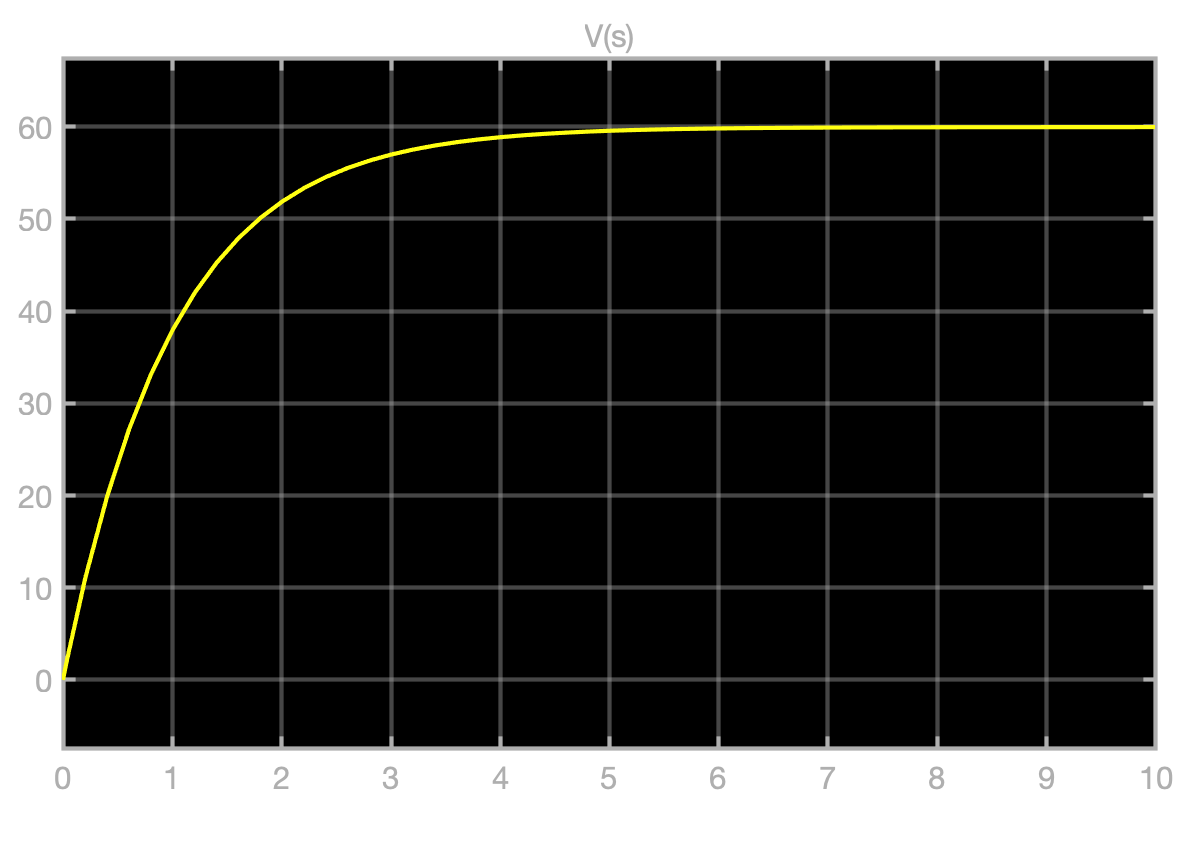
\includegraphics[width=0.6\linewidth]{Bilder/P_Reg_Tracking.eps}
	\caption{Tracking achieved by Hight Propotional controller gain}
	\label{Fig_P_Regulator_Tracking}
\end{figure}

\subsection{Effects of Noise with Proportional Regulator} \label{Sec_NoiseInClosedloopArchitecture}

With noise as the input signal (ignoring $R(s)$) the closed loop TF of the system is expressed as:
\begin{equation} \label{Eq_CL_Noise}
	\frac{V(s)}{N(s)} = \frac{-\frac{K}{ms + b}}{1 + \frac{K}{ms + b}} = \frac{-K}{ms + b + K}
\end{equation}

From equation \ref{Eq_CL_Noise}m it can be seen that when $K$ is made sufficiently large, the TF will increase towards a value of $-1$. A TF of $-1$ will make the system output $V(s)$ react to noise in the opposite to the desired value and it amplifies as $K$ increases. Therefore, a larger $K$ will amplify the effect of noises into the system and such cases the system will fail to track as shown in figure \ref{Fig_P_Regulator_Tracking_Noise}.
\begin{figure}[h!]
	\centering
	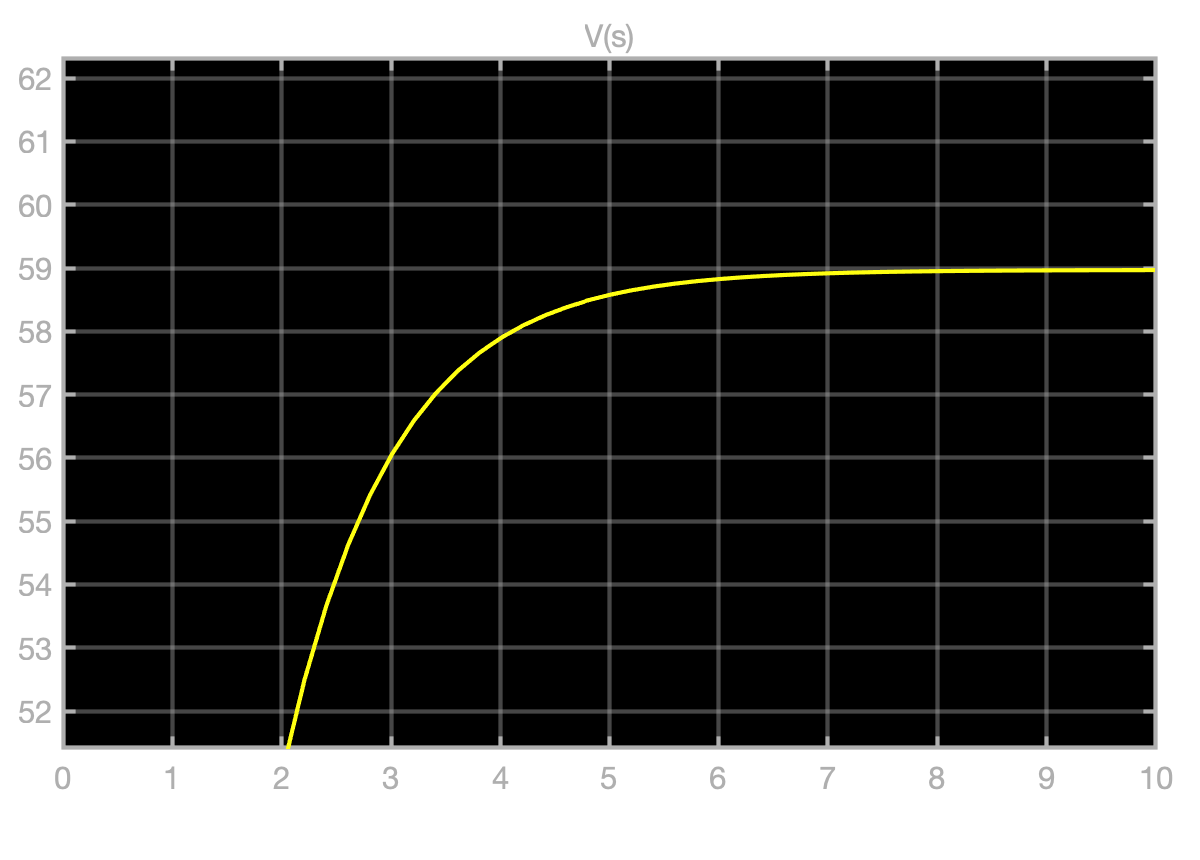
\includegraphics[width=0.6\linewidth]{Bilder/P_Reg_with_Noise.eps}
	\caption{Tracking failed by high Proportional controller gain with noise}
	\label{Fig_P_Regulator_Tracking_Noise}
\end{figure}

Additionally, there is also something called actuator saturation that comes from larger $K$ ie., limit of engine dynamics, friction between tire-road interface among others which would lead to higher fuel consumption among others. Additionally a larger $K$ will induce system oscillations. Therefore, it is necessary to avoid larger $K$ due to noise disturbance amplifications, actuator saturation and system oscillations (due to overshoot).








